\documentclass[11pt]{article}

\usepackage[UTF8]{ctex}
\usepackage[a4paper]{geometry}
\usepackage{amsmath}
\usepackage{fancyhdr}
\usepackage{amsthm}
\usepackage{amssymb}
\usepackage{xcolor}
\usepackage{tikzsymbols}
\usepackage{gensymb}
\usepackage{ctex} % 支持中文的LaTeX宏包
\usepackage{amsmath,amsfonts,graphicx,subfigure,amssymb,bm,amsthm,mathrsfs,mathtools,breqn} % 数学公式和符号的宏包集合
\usepackage{algorithm,algorithmicx} % 算法和伪代码
\usepackage[noend]{algpseudocode} % 算法和伪代码
\usepackage{fancyhdr} % 自定义页眉页脚
\usepackage[framemethod=TikZ]{mdframed} % 创建带边框的框架
\usepackage{fontspec} % 字体设置
\usepackage{adjustbox} % 调整盒子大小
\usepackage{fontsize} % 设置字体大小
\usepackage{tikz,xcolor} % 绘制图形和使用颜色
\usepackage{multicol} % 多栏排版
\usepackage{multirow} % 表格中合并单元格
\usepackage{pdfpages} % 插入PDF文件
\usepackage{listings} % 在文档中插入源代码
\usepackage{wrapfig} % 文字绕排图片
\usepackage{bigstrut,multirow,rotating} % 支持在表格中使用特殊命令
\usepackage{booktabs} % 创建美观的表格
\usepackage{circuitikz} % 绘制电路图
\usepackage{zhnumber} % 中文序号(用于标题)
\usepackage{tabularx} % 表格折行
\usepackage{titlesec}
\usepackage{slashbox}
\newcolumntype{C}[1]{>{\centering\arraybackslash}p{#1}} %定义居中的列
\definecolor{CPPLight}  {HTML} {686868}
\definecolor{CPPSteel}  {HTML} {888888}
\definecolor{CPPDark}   {HTML} {262626}
\definecolor{CPPBlue}   {HTML} {4172A3}
\definecolor{CPPGreen}  {HTML} {487818}
\definecolor{CPPBrown}  {HTML} {A07040}
\definecolor{CPPRed}    {HTML} {AD4D3A}
\definecolor{CPPViolet} {HTML} {7040A0}
\definecolor{CPPGray}  {HTML} {B8B8B8}
\lstset{
    columns=fixed,       
    numbers=left,                                        % 在左侧显示行号
    frame=none,                                          % 不显示背景边框
    backgroundcolor=\color[RGB]{245,245,244},            % 设定背景颜色
    keywordstyle=\color[RGB]{40,40,255},                 % 设定关键字颜色
    numberstyle=\footnotesize\color{darkgray},           % 设定行号格式
    commentstyle=\it\color[RGB]{0,96,96},                % 设置代码注释的格式
    stringstyle=\rmfamily\slshape\color[RGB]{128,0,0},   % 设置字符串格式
    showstringspaces=false,                              % 不显示字符串中的空格
    language={[x86masm]Assembler},                       % 改为x86-32汇编高亮
    morekeywords={mull, divl, addb leal,xorl,pushl,popl,testl,testb,movl,movb,incl,decl,cmpb,cmpl,mov,add,sub,jmp,cmp,je,jne,push,pop,inc,dec,call,ret,lea,nop,or,and,xor,int,syscall,sysreturn},
    emph={eax,ebx,ecx,edx,esi,edi,esp,ebp,eip},
    emphstyle=\color{CPPViolet},
}



\titleformat{\section}{\fontsize{20pt}{22pt}\selectfont\bfseries}{\thesection}{1em}{}
\titleformat{\subsection}{\fontsize{18pt}{20pt}\bfseries}{\thesubsection}{1em}{}
\titleformat{\subsubsection}{\fontsize{16pt}{18pt}\bfseries}{\thesubsubsection}{1em}{}


\definecolor{dkgreen}{rgb}{0,0.6,0}
\definecolor{gray}{rgb}{0.5,0.5,0.5}
\definecolor{mauve}{rgb}{0.58,0,0.82}
\lstset{
  frame=tb,
  aboveskip=3mm,
  belowskip=3mm,
  showstringspaces=false,
  columns=flexible,
  framerule=1pt,
  rulecolor=\color{gray!35},
  backgroundcolor=\color{gray!5},
  basicstyle={\small\ttfamily},
  numbers=left,
  numberstyle=\color{gray},
  keywordstyle=\color{blue},
  commentstyle=\color{dkgreen},
  stringstyle=\color{mauve},
  breaklines=true,
  breakatwhitespace=true,
  tabsize=3,
}
\setlength{\headheight}{14.49998pt}

\newtheorem{question}{\hskip 1.7mm \bf}
\renewenvironment{proof}{{\noindent\hskip 2.4em \bf ֤证明 \quad}}{\hfill$\qed$\par}
\newenvironment{solution}{{\noindent\hskip 2.4em \bf 解 \quad}}


\geometry{left=2.0cm,right=2.0cm,top=2.5cm,bottom=2.5cm}
\begin{document}
\fontsize{13pt}{18pt}\selectfont

\pagestyle{fancy}
\lhead{中国科学院大学}
\chead{\bf{汇编语言}}
\rhead{\emph{薛翼舟}}


\begin{center}
\huge{\bf{《汇编语言》大作业2-矩阵乘法的优化}}
\end{center}

在本次作业中, 我一共采用了共5中方法来优化计算, 下面逐个讲解, 有关运行时间的计算, 我在本地运行时发现
每次运算的时间方差较大, 于是我擦爱用了计算7次, 去掉其中的最大值和最小值, 求平均的办法来相对严谨地计算运行时间

\section{Python原始代码}

{\setmainfont{Courier New Bold}                          % 设置代码字体                   
    \begin{lstlisting}[language=Python]
import numpy as np
import time

N = 4096
A = np.random.randint(0, 10, (N, N), dtype=np.int32)
B = np.random.randint(0, 10, (N, N), dtype=np.int32)
C = np.zeros((N, N), dtype=np.int32)

start = time.time()
for i in range(N):
    for j in range(N):
        for k in range(N):
            C[i, j] += A[i, k] * B[k, j]
end = time.time()
print("Python naive time:", end - start)
\end{lstlisting}}
这是最原始的python代码, 由于这次矩阵的大小为4096, 所以计算量非常大, 直接运行会花费很长时间, 大约花费了35小时,大约126000秒(这个数字是根据小规模的矩阵推算得到, 可能并不准确)

\section{线性计算的C代码}

{\setmainfont{Courier New Bold}                                        
    \begin{lstlisting}[language=C]
#include <stdio.h>
#include <stdlib.h>
#include <time.h>

#define N 4096

//最基本的矩阵乘法函数, 逐个行列相乘
void matrixmultiply(int n, int **A, int **B, int **C) {
    for (int i = 0; i < n; ++i)
        for (int j = 0; j < n; ++j) {
            int sum = 0;
            for (int k = 0; k < n; ++k)
                sum += A[i][k] * B[k][j];
            C[i][j] = sum;
        }
}

int main() {
  //为ABC分配内存空间
    int **A = malloc(N * sizeof(int*));
    int **B = malloc(N * sizeof(int*));
    int **C = malloc(N * sizeof(int*));
    for (int i = 0; i < N; ++i) {
        A[i] = malloc(N * sizeof(int));
        B[i] = malloc(N * sizeof(int));
        C[i] = malloc(N * sizeof(int));
        for (int j = 0; j < N; ++j) {
            A[i][j] = rand() % 10;
            B[i][j] = rand() % 10;
        }
    }
    clock_t start = clock();
    matrixmultiply(N, A, B, C);
    clock_t end = clock();
    printf("Serial time: %.2f seconds\n", (double)(end - start) / CLOCKS_PER_SEC);
  //释放内存
    for (int i = 0; i < N; ++i) {
        free(A[i]); free(B[i]); free(C[i]);
    }
    free(A); free(B); free(C);
}
\end{lstlisting}}
部分运行截图如下
\begin{figure}[H]
    \centering
    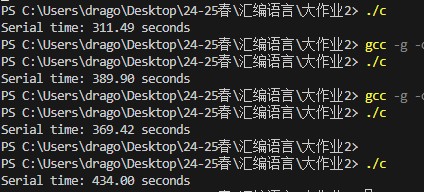
\includegraphics[width=0.8\textwidth]{c.png}
    \caption{线性计算的C代码部分运行截图}
\end{figure}
以下是7次运行中选取的5次有效时间的表格
 \begin{table}[H]
        \centering
        \begin{tabular}{|c|C{2cm}|C{2cm}|C{2cm}|C{2cm}|C{2cm}|}\hline
            运行编号 & 1 & 2 & 3 & 4 & 5 \\\hline
            运行时间(s) & 311.50 & 389.90 & 369.42 & 401.27 & 352.89\\\hline
            平均时间(s) & \multicolumn{5}{|c|}{364.99} \\\hline
        \end{tabular}  
  \end{table}
这个程序是很平凡的想法, 在此不多赘述

\section{矩阵分块计算}
由于之后的几个哈桉树中main函数的差意不大, 所以在此将相同的main函数和宏定义省去
{\setmainfont{Courier New Bold}                                        
    \begin{lstlisting}[language=C]
#define BLOCK 128

void matrixmultiply(int n, int **A, int **B, int **C) {
    for (int ii = 0; ii < n; ii += BLOCK)
        for (int jj = 0; jj < n; jj += BLOCK)
            for (int kk = 0; kk < n; kk += BLOCK)
                for (int i = ii; i < ii + BLOCK && i < N; ++i)
                    for (int j = jj; j < jj + BLOCK && j < N; ++j) {
                        int sum = 0;
                        for (int k = kk; k < kk + BLOCK && k < N; ++k)
                            sum += A[i][k] * B[k][j];
                        C[i][j] += sum;
                    }
}
\end{lstlisting}}
在这个代码中我们可以看到, 我们将整个大的矩阵拆分为几个小的块, 每次计算一个小块的矩阵, 这样可以减少缓存未命中的次数, 
提高计算速度, 这个BLOCK的大小是根据我们的cache自定的, 所以这个BLOCK的大小要根据不同的输入规模和不同的计算机进行调整,
在我的计算机上, 我测试了几个不同的BLOCK值(16,32,64,256), 我发现128和256的加速效果最好, 而且二者相差不多, 我选取了128\par
以下是部分代码运行截图
\begin{figure}[H]
    \centering
    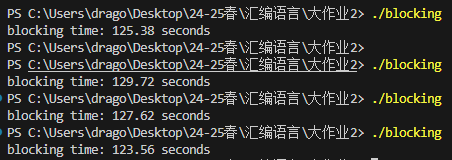
\includegraphics[width=0.8\textwidth]{block.jpg}
    \caption{矩阵分块计算的C代码部分运行截图}
\end{figure}
以下是7次运行中选取的5次有效时间的表格
 \begin{table}[H]
        \centering
        \begin{tabular}{|c|C{2cm}|C{2cm}|C{2cm}|C{2cm}|C{2cm}|}\hline
            运行编号 & 1 & 2 & 3 & 4 & 5 \\\hline
            运行时间(s) & 125.38 & 129.72 & 127.42 & 123.56 & 120.29\\\hline
            平均时间(s) & \multicolumn{5}{|c|}{125.27} \\\hline
        \end{tabular}  
  \end{table}

\section{多核多线程加速}
{\setmainfont{Courier New Bold}                                        
    \begin{lstlisting}[language=C]
#include <omp.h>

void matrixmultiply(int n, int **A, int **B, int **C) {
    #pragma omp parallel for
    for (int i = 0; i < n; ++i)
        for (int j = 0; j < n; ++j) {
            int sum = 0;
            for (int k = 0; k < n; ++k)
                sum += A[i][k] * B[k][j];
            C[i][j] = sum;
        }
}
\end{lstlisting}}
我们的并行多线程中, 对于C程序没有改变, 就是多了如下指令
{\setmainfont{Courier New Bold}                                        
    \begin{lstlisting}[language=C]
#pragma omp parallel for
\end{lstlisting}}
这条指令的作用是告诉编译器创建一组等于我计算机核心数的线程, 并且将接下来的for循环中的迭代空间自动划分给这些线程,
实际上就是将串行的运作转为多个线程并行的工作, 我们在命令
{\setmainfont{Courier New Bold}                                        
    \begin{lstlisting}[language=C]
gcc -S -fopenmp -mavx2 -mfma -o openmp.s openmp.c
\end{lstlisting}}
下所得到的.s文件中可以看到如下命令
{\setmainfont{Courier New Bold}                                        
    \begin{lstlisting}
call	omp_get_num_threads
call	omp_get_thread_num


\end{lstlisting}}  
代表调用多核多线程来解决串行的循环\par
以下是部分代码运行截图
\begin{figure}[H]
    \centering
    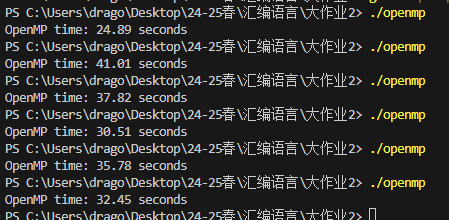
\includegraphics[width=0.8\textwidth]{openmp.png}
    \caption{多核多线程加速的C代码部分运行截图}
\end{figure}
以下是7次运行中选取的5次有效时间的表格
 \begin{table}[H]
        \centering
        \begin{tabular}{|c|C{2cm}|C{2cm}|C{2cm}|C{2cm}|C{2cm}|}\hline
            运行编号 & 1 & 2 & 3 & 4 & 5 \\\hline
            运行时间(s) & 37.82 & 30.51 & 35.78 & 32.45 & 31.98\\\hline
            平均时间(s) & \multicolumn{5}{|c|}{33.71} \\\hline
        \end{tabular}  
  \end{table}


\section{SIMD指令集和多核多线程加速}
{\setmainfont{Courier New Bold}                                        
    \begin{lstlisting}[language=C]
#include <immintrin.h>
#include <stdio.h>
#include <stdlib.h>
#include <time.h>
#include <omp.h>

#define N 4096

void matrixmultiply(int n, float **A, float **B, float **C) {
    #pragma omp parallel for
    for (int i = 0; i < n; ++i)
        for (int j = 0; j < n; ++j) {
            __m256 sum = _mm256_setzero_ps();
            for (int k = 0; k < N; k += 8) {
                __m256 a = _mm256_loadu_ps(&A[i][k]);
                __m256 b = _mm256_loadu_ps(&B[k][j]);
                sum = _mm256_fmadd_ps(a, b, sum);
            }
            float tmp[8];
            _mm256_storeu_ps(tmp, sum);
            float total = 0;
            for (int x = 0; x < 8; ++x) total += tmp[x];
            C[i][j] = total;
        }
}

int main() {
    float **A = (float**)malloc(N * sizeof(float*));
    float **B = (float**)malloc(N * sizeof(float*));
    float **C = (float**)malloc(N * sizeof(float*));
    for (int i = 0; i < N; ++i) {
        A[i] = (float*)malloc(N * sizeof(float));
        B[i] = (float*)malloc(N * sizeof(float));
        C[i] = (float*)calloc(N, sizeof(float));
        for (int j = 0; j < N; ++j) {
            A[i][j] = (float)(rand() % 10);
            B[i][j] = (float)(rand() % 10);
        }
    }
    clock_t start = clock();
    matrixmultiply(N, A, B, C);
    clock_t end = clock();
    printf("SIMD time: %.2f seconds\n", (double)(end - start) / CLOCKS_PER_SEC);

    for (int i = 0; i < N; ++i) {
        free(A[i]); free(B[i]); free(C[i]);
    }
    free(A); free(B); free(C);

    return 0;
}
\end{lstlisting}}
在这里由于使用了SIMD指令集, 因此为我们改用了float型, 其中比较关键的是标识符\__m256, 这个代表我们使用了256位的向量寄存器, 
可以同时处理8个float类型的数据, 从而实现数据的并行处理. 我们应该用碧嘉澳查昂的寄存器来尽可能的用我们并行所得到的提升来覆盖
生成寄存器的开销, 这样才能得到更好的性能提升, 在这里我们使用了\_mm256\_loadu\_ps和\_mm256\_storeu\_ps来加载和存储数据,
同时使用\_mm256\_fmadd\_ps来进行乘加操作, 这样可以减少指令的数量, 提高计算效率. 在汇编中我们发现了形如
{\setmainfont{Courier New Bold}                                        
    \begin{lstlisting}
	vmovups	(%rax), %ymm0
	vmovups	%ymm0, 128(%rbx)
	vmovups	160(%rbx), %ymm0
	vmovups	%ymm0, 64(%rbx)
	vmovups	128(%rbx), %ymm0
	vmovups	%ymm0, 32(%rbx)
	vmovups	192(%rbx), %ymm0
	vmovups	%ymm0, (%rbx)
	vmovups	32(%rbx), %ymm1
	vmovups	(%rbx), %ymm0
	vfmadd231ps	64(%rbx), %ymm1, %ymm0
\end{lstlisting}}
的关键汇编指令, 我们并行地同时处理了很多组数据, 大大提升了效率\par
以下是部分代码运行截图
\begin{figure}[H]
    \centering
    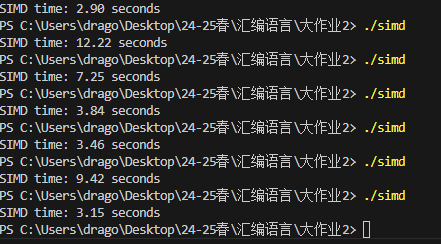
\includegraphics[width=0.8\textwidth]{simd.png}
    \caption{SIMD指令集加速的C代码部分运行截图}
\end{figure} 

以下是7次运行中选取的5次有效时间的表格
 \begin{table}[H]
        \centering
        \begin{tabular}{|c|C{2cm}|C{2cm}|C{2cm}|C{2cm}|C{2cm}|}\hline
            运行编号 & 1 & 2 & 3 & 4 & 5 \\\hline
            运行时间(s) & 7.25 & 3.84 & 3.46 & 9.42 & 3.15\\\hline
            平均时间(s) & \multicolumn{5}{|c|}{5.82} \\\hline
        \end{tabular}  
  \end{table}
我们发现SIMD程序所得到的运行时间的方差比较大,个人猜测是simd指令这种运算方法和多核多线程的方式
对于输入的数据比较敏感

\section{其他加速方法-Strassen算法}
Strassen算法的核心思想是将大矩阵分解为小矩阵, 来通过减少乘法次数来降低计算复杂度, 
最终可以达到$O(n^{\log_2 7}) \approx O(n^{2.81})$的复杂度, 但是代码实现很复杂, 代码如下
{\setmainfont{Courier New Bold}                                        
    \begin{lstlisting}
#define THRESHOLD 64  // 小于此尺寸时用普通乘法

void classic_multiply(int n, int **A, int **B, int **C) {
    for (int i=0; i<n; ++i)
        for (int j=0; j<n; ++j)
            for (int k=0; k<n; ++k)
                C[i][j] += A[i][k] * B[k][j];
}

void add(int n, int **A, int **B, int **C) {
    for (int i=0; i<n; ++i)
        for (int j=0; j<n; ++j)
            C[i][j] = A[i][j] + B[i][j];
}

void sub(int n, int **A, int **B, int **C) {
    for (int i=0; i<n; ++i)
        for (int j=0; j<n; ++j)
            C[i][j] = A[i][j] - B[i][j];
}

void strassen(int n, int **A, int **B, int **C) {
    if (n <= THRESHOLD) {
        classic_multiply(n, A, B, C);
        return;
    }
    int k = n/2;
    // Allocate submatrices
    int **A11 = malloc(k*sizeof(int*));
    int **A12 = malloc(k*sizeof(int*));
    int **A21 = malloc(k*sizeof(int*));
    int **A22 = malloc(k*sizeof(int*));
    int **B11 = malloc(k*sizeof(int*));
    int **B12 = malloc(k*sizeof(int*));
    int **B21 = malloc(k*sizeof(int*));
    int **B22 = malloc(k*sizeof(int*));
    int **C11 = malloc(k*sizeof(int*));
    int **C12 = malloc(k*sizeof(int*));
    int **C21 = malloc(k*sizeof(int*));
    int **C22 = malloc(k*sizeof(int*));
    for (int i=0; i<k; ++i) {
        A11[i] = A[i];
        A12[i] = A[i] + k;
        A21[i] = A[i+k];
        A22[i] = A[i+k] + k;
        B11[i] = B[i];
        B12[i] = B[i] + k;
        B21[i] = B[i+k];
        B22[i] = B[i+k] + k;
        C11[i] = C[i];
        C12[i] = C[i] + k;
        C21[i] = C[i+k];
        C22[i] = C[i+k] + k;
    }
    // Allocate temp matrices
    int **M1 = malloc(k*sizeof(int*));
    int **M2 = malloc(k*sizeof(int*));
    int **M3 = malloc(k*sizeof(int*));
    int **M4 = malloc(k*sizeof(int*));
    int **M5 = malloc(k*sizeof(int*));
    int **M6 = malloc(k*sizeof(int*));
    int **M7 = malloc(k*sizeof(int*));
    int **T1 = malloc(k*sizeof(int*));
    int **T2 = malloc(k*sizeof(int*));
    for (int i=0; i<k; ++i) {
        M1[i] = calloc(k, sizeof(int));
        M2[i] = calloc(k, sizeof(int));
        M3[i] = calloc(k, sizeof(int));
        M4[i] = calloc(k, sizeof(int));
        M5[i] = calloc(k, sizeof(int));
        M6[i] = calloc(k, sizeof(int));
        M7[i] = calloc(k, sizeof(int));
        T1[i] = calloc(k, sizeof(int));
        T2[i] = calloc(k, sizeof(int));
    }
    // M1 = (A11 + A22)*(B11 + B22)
    add(k, A11, A22, T1);
    add(k, B11, B22, T2);
    strassen(k, T1, T2, M1);
    // M2 = (A21 + A22)*B11
    add(k, A21, A22, T1);
    strassen(k, T1, B11, M2);
    // M3 = A11*(B12 - B22)
    sub(k, B12, B22, T2);
    strassen(k, A11, T2, M3);
    // M4 = A22*(B21 - B11)
    sub(k, B21, B11, T2);
    strassen(k, A22, T2, M4);
    // M5 = (A11 + A12)*B22
    add(k, A11, A12, T1);
    strassen(k, T1, B22, M5);
    // M6 = (A21 - A11)*(B11 + B12)
    sub(k, A21, A11, T1);
    add(k, B11, B12, T2);
    strassen(k, T1, T2, M6);
    // M7 = (A12 - A22)*(B21 + B22)
    sub(k, A12, A22, T1);
    add(k, B21, B22, T2);
    strassen(k, T1, T2, M7);
    // C11 = M1 + M4 - M5 + M7
    for (int i=0; i<k; ++i)
        for (int j=0; j<k; ++j)
            C11[i][j] = M1[i][j] + M4[i][j] - M5[i][j] + M7[i][j];
    // C12 = M3 + M5
    for (int i=0; i<k; ++i)
        for (int j=0; j<k; ++j)
            C12[i][j] = M3[i][j] + M5[i][j];
    // C21 = M2 + M4
    for (int i=0; i<k; ++i)
        for (int j=0; j<k; ++j)
            C21[i][j] = M2[i][j] + M4[i][j];
    // C22 = M1 - M2 + M3 + M6
    for (int i=0; i<k; ++i)
        for (int j=0; j<k; ++j)
            C22[i][j] = M1[i][j] - M2[i][j] + M3[i][j] + M6[i][j];
    // Free allocated memory
    for (int i=0; i<k; ++i) {
        free(M1[i]); free(M2[i]); free(M3[i]); free(M4[i]);
        free(M5[i]); free(M6[i]); free(M7[i]);
        free(T1[i]); free(T2[i]);
    }
    free(A11); free(A12); free(A21); free(A22);
    free(B11); free(B12); free(B21); free(B22);
    free(C11); free(C12); free(C21); free(C22);
    free(M1); free(M2); free(M3); free(M4); free(M5); free(M6); free(M7);
    free(T1); free(T2);
}
\end{lstlisting}}
这个算法的实现是网上查阅资料所的得到的, 核心思想就是利用矩阵分块, 来一定程度上减少乘法的次数\par
以下是部分代码运行截图
\begin{figure}[H]
    \centering
    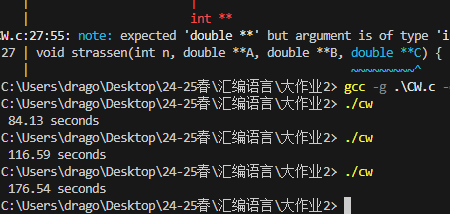
\includegraphics[width=0.8\textwidth]{strassen.png}
    \caption{Strassen算法的C代码部分运行截图}
\end{figure}
以下是7次运行中选取的5次有效时间的表格
 \begin{table}[H]
        \centering
        \begin{tabular}{|c|C{2cm}|C{2cm}|C{2cm}|C{2cm}|C{2cm}|}\hline
            运行编号 & 1 & 2 & 3 & 4 & 5 \\\hline
            运行时间(s) & 116.59 & 123.23 & 136.12 & 120.42 & 131.74\\\hline
            平均时间(s) & \multicolumn{5}{|c|}{125.42} \\\hline
        \end{tabular}  
  \end{table}

\section{总结}
\subsection{加速比}
在本次作业中, 我们通过多种方法来优化矩阵乘法的计算, 包括线性计算、矩阵分块计算、多核多线程加速、SIMD指令集和Strassen算法等,
我们利用$rate = \frac{T_{py}}{T}$来计算如上5个加速算法的加速比, 由于python基础算法的时间过长, 我们在此不做计算, 以线性
矩阵计算作为基准值
\begin{table}[H]
    \centering
    \begin{tabular}{|c|C{2cm}|C{2cm}|C{2cm}|C{2cm}|C{2.4cm}|}\hline
        方法 & 线性计算 & 矩阵分块 & 多核多线程 & SIMD指令集+多核多线程 & Strassen算法 \\\hline
        运行时间(s) & 364.99 & 125.27 & 33.71 & 5.82 & 125.42 \\\hline
        加速比 & 1.00 & 2.91 & 10.85 & 62.70 & 2.91 \\\hline
    \end{tabular}
\end{table}
我们可以看到, SIMD指令集和多核多线程的结合使用, 在加速比上达到了62.70, 充分利用了硬件资源, 提高了计算效率.
\subsection{加速瓶颈}
综合我们上面的几种加速方法的原理和效果, 我认为有如下加速瓶颈
\begin{enumerate}
  \item 矩阵分块的大小选择对性能影响较大, 需要根据具体硬件进行调优
  \item 在多核多线程中, 线程的个数以及线程之间的通信和同步开销会影响性能
  \item SIMD指令集能否用更长的寄存器?
\end{enumerate}
\end{document}